\begin{multicols}{2}
\section{Interfacing With the Sensor}
The sensor contains two interfaces. One for using the sensor and one for programming the sensor.
\subsection{Main interface}
The main interface is used for powering the sensor, communication (\iic) and interrupts.
\begin{figure}[H]
 \centering
 
\includegraphics[width=0.2\textwidth]{../img/J2.png}
\end{figure}

\begin{description}
	\item[Power] (Pins \texttt{VCC} and \texttt{GND}) \\
	Sensor can be powered from any source ranging from 3.0V to 5.5V connected to \texttt{VCC}. Connect \texttt{GND} to ground. 
	
	\item[\iic] (Pins \texttt{SCL} and \texttt{SDA}) \\
	\iic port. Connect sensor \texttt{SCL} to master \texttt{SCL} and sensor \texttt{SDA} to master \texttt{SDA}.\\
	Compatibility : \cite{i2cspec} \cite{microchipDS}
	\begin{itemize}
		\item standard mode (100kbit/s)
		\item fast mode (400kbit/s)
	\end{itemize}
	
	\item[Interrupts] (Pin \texttt{INT}) \\
	Interrupts output. Pin is driven low when an interrupt is triggered and reset to high when a data register is read.
\end{description}
	\textit{\textbf{Note:} On PCB V1.0 interrupts only works if the sensor is powered with 3.0V-3.3V.}

%\columnbreak

\subsection{Programming interface}
\begin{figure}[H]
 \centering
 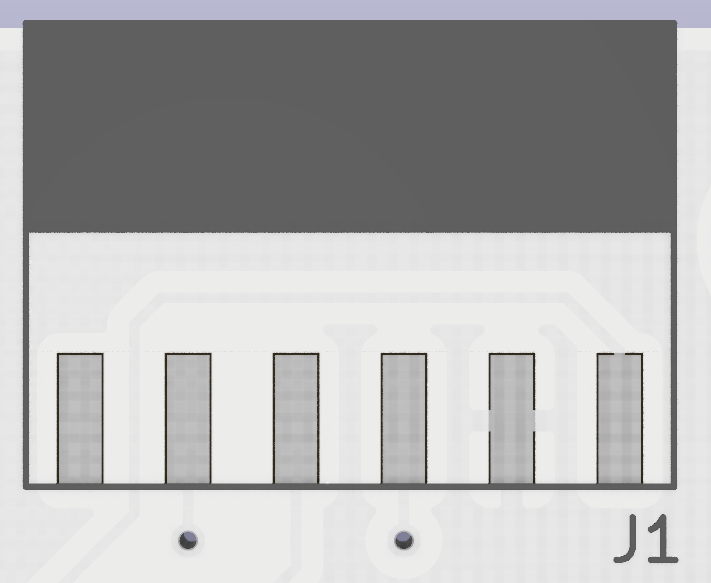
\includegraphics[width=0.2\textwidth]{../img/J1.png}
\end{figure}

	That is the \texttt{ICSP} header used to reprogram the PIC firmware.
	
	\textit{\textbf{Note:} On PCB V1.0 the connector is not keyed. VPP is connected to the pin on the right of the picture.}
	
	\textit{\textbf{Note:} On PCB V1.0 the \texttt{VCC} pin is directly connected to the internal power rail of the sensor. Components on the board are rated to 3.3V and will not tolerate more. Caution must be used when reprogramming the board to not apply more than 3.3V. Advice is to configure the programmer so that it does not power the sensor. Provide the required power via the main interface \texttt{J2}.}
	
\end{multicols}